\chapter{NoSQL dan Data Semi-Struktur}

\section{Background}

Dalam era digital saat ini, volume, kecepatan, dan variasi data terus meningkat secara eksponensial. Konsep ini pertama kali diperkenalkan oleh Laney (2001) melalui framework 3V: Volume, Velocity, Variety \cite{laney2001}, yang kemudian menjadi dasar pemahaman big data di dunia bisnis dan teknologi. Basis data relasional (RDBMS) telah lama menjadi standar utama untuk menyimpan dan mengelola data terstruktur. Namun, keterbatasan RDBMS mulai terlihat ketika organisasi menghadapi kebutuhan untuk menyimpan data dalam skala besar, dengan struktur yang tidak selalu terdefinisi dengan ketat, dan kebutuhan ketersediaan tinggi di lingkungan terdistribusi \cite{stonebraker2010sql, kimball2013}.

Untuk mengatasi keterbatasan ini, muncul paradigma \textbf{NoSQL} (Not Only SQL), yang menawarkan pendekatan penyimpanan dan pengelolaan data dengan fleksibilitas skema lebih tinggi, performa baca-tulis cepat, serta kemampuan untuk diskalakan secara horizontal di banyak server \cite{han2011survey}. NoSQL mendukung penyimpanan data semi-struktur dan tidak terstruktur seperti JSON, yang kini banyak digunakan dalam aplikasi web modern, e-commerce, media sosial, serta sistem IoT \cite{gandomi2015}.

Selain itu, konsep \textbf{CAP theorem} yang diperkenalkan oleh Brewer menegaskan adanya trade-off antara Consistency, Availability, dan Partition Tolerance dalam sistem terdistribusi \cite{brewer2012cap}. Pemahaman akan hal ini penting bagi manajer dan profesional bisnis saat memilih teknologi basis data untuk mendukung kebutuhan operasional dan strategis organisasi.

Dengan demikian, bab ini akan membahas konsep NoSQL, alasan kemunculannya, tipe-tipe utama NoSQL seperti Document Database dan Graph Database, serta relevansinya dalam mendukung fleksibilitas dan skalabilitas sistem informasi bisnis modern.


\section{Konsep Data Semi-Struktur}

\subsection{Definisi dan Karakteristik}

Data semi-struktur adalah jenis data yang tidak disimpan dalam skema tabel relasional yang kaku, namun memiliki tag, marker, atau struktur hierarkis yang memungkinkan interpretasi data oleh mesin maupun manusia. Berbeda dengan data terstruktur (misalnya tabel RDBMS) yang memiliki skema tetap dan rigid, data semi-struktur memungkinkan fleksibilitas dalam penambahan atribut baru tanpa harus mengubah definisi skema secara keseluruhan \cite{gandomi2015, moniruzzaman2013nosql}.

Menurut \cite{moniruzzaman2013nosql}, data semi-struktur memiliki karakteristik utama sebagai berikut:
\begin{enumerate}
	\item \textbf{Schema-on-read:} tidak memerlukan skema tetap sebelum data disimpan, melainkan skema diterapkan saat data dibaca untuk analisis.
	\item \textbf{Struktur hierarkis dan fleksibel:} data disimpan dalam nested structures (struktur bersarang) yang mendukung kompleksitas relasi antar atribut.
	\item \textbf{Format berbasis teks dan kunci-nilai:} umumnya mudah diproses oleh mesin dan tetap dapat dibaca manusia.
	\item \textbf{Extensible:} mudah menambahkan atribut baru tanpa memengaruhi data existing.
\end{enumerate}

Contoh paling umum dari data semi-struktur adalah \textbf{JSON (JavaScript Object Notation)}, \textbf{XML (eXtensible Markup Language)}, dan \textbf{YAML (YAML Ain't Markup Language)}. Format ini mendukung fleksibilitas tinggi sehingga banyak digunakan dalam penyimpanan data konfigurasi, pertukaran data via API, serta integrasi antar sistem yang heterogen \cite{han2011survey}.

Dalam konteks bisnis modern, data semi-struktur menjadi penting karena:
\begin{itemize}
	\item Mendukung integrasi data dari berbagai sumber dengan format berbeda tanpa perlu transformasi awal yang kompleks.
	\item Mempercepat pengembangan aplikasi digital (agile development) dengan memungkinkan skema yang dinamis.
	\item Memudahkan pemrosesan data unstructured dan semi-structured dalam big data analytics \cite{gandomi2015}.
\end{itemize}

\subsection{Contoh Format Data Semi-Struktur}

\textbf{JSON} adalah format data semi-struktur yang paling banyak digunakan dalam aplikasi web, mobile, dan layanan cloud modern. Contoh JSON dalam konteks e-commerce dapat berupa data produk berikut:

\begin{lstlisting}[language=json, caption={Contoh struktur data produk dalam format JSON}, label={lst:json_product}]
	{
		"id": 101,
		"name": "Laptop ASUS VivoBook",
		"category": "Electronics",
		"price": 8500000,
		"specs": {
			"processor": "Intel i5",
			"ram": "8GB",
			"storage": "512GB SSD"
		},
		"tags": ["laptop", "asus", "notebook", "electronics"]
	}
\end{lstlisting}

Contoh di atas menunjukkan bagaimana JSON dapat menyimpan data produk dengan atribut sederhana (id, name, category, price) sekaligus menyertakan nested object (specs) dan array (tags). Format ini mendukung fleksibilitas tinggi dan memudahkan integrasi antar layanan melalui RESTful API.

Selain JSON, format semi-struktur lain yang relevan dalam bisnis meliputi:
\begin{itemize}
	\item \textbf{XML}: banyak digunakan dalam integrasi sistem enterprise, khususnya pada SOAP web services dan dokumen standar industri.
	\item \textbf{YAML}: populer untuk konfigurasi aplikasi, deployment DevOps (misalnya Kubernetes manifest files), dan pipeline CI/CD karena lebih ringkas dibanding XML.
\end{itemize}

Menurut \cite{moniruzzaman2013nosql, gandomi2015}, penggunaan data semi-struktur terus meningkat seiring dengan kebutuhan integrasi data lintas platform dan pengembangan aplikasi yang agile. Data semi-struktur memberikan keseimbangan antara struktur dan fleksibilitas, sehingga menjadi fondasi penting dalam arsitektur big data modern.



\section{Pengenalan NoSQL}

\subsection{Definisi dan Motivasi Bisnis}

\textbf{NoSQL}, atau \emph{Not Only SQL}, adalah istilah untuk teknologi basis data non-relasional yang dirancang untuk mengatasi keterbatasan RDBMS dalam menghadapi tantangan big data modern. Berbeda dengan RDBMS yang menggunakan tabel dengan skema tetap, NoSQL mendukung penyimpanan data dalam format fleksibel seperti dokumen JSON, key-value, graph, dan wide-column store \cite{han2011survey, stonebraker2010sql, moniruzzaman2013nosql}.

Menurut \cite{moniruzzaman2013nosql}, terdapat empat motivasi utama munculnya NoSQL:

\begin{enumerate}
	\item \textbf{Scalability (Skalabilitas Horizontal)}  
	RDBMS tradisional cenderung dioptimasi untuk scale-up, yaitu peningkatan kapasitas server tunggal. NoSQL mendukung \emph{scale-out} melalui distribusi data ke beberapa server (sharding), sehingga biaya lebih rendah dan performa lebih tinggi ketika data tumbuh eksponensial, misalnya pada aplikasi media sosial atau IoT.
	
	\item \textbf{Flexibility (Fleksibilitas Skema)}  
	NoSQL mendukung struktur data dinamis atau semi-struktur tanpa skema tetap (schema-less). Hal ini penting untuk bisnis yang mengimplementasikan \emph{agile development}, di mana kebutuhan fitur sering berubah, sehingga skema data dapat disesuaikan tanpa migrasi kompleks \cite{han2011survey}.
	
	\item \textbf{High Performance and Availability}  
	NoSQL dioptimasi untuk latensi rendah dan throughput tinggi, mendukung use case real-time analytics, caching session user, dan streaming data dalam skala besar \cite{gandomi2015, stonebraker2018sql}.
	
	\item \textbf{Handling Unstructured and Semi-Structured Data}  
	Seiring meningkatnya data semi-struktur (JSON, XML) dan tidak terstruktur (teks, gambar, video) dari e-commerce, media sosial, dan log aplikasi, NoSQL menawarkan cara penyimpanan yang lebih natural dan hemat waktu dibanding memaksakan normalisasi ke tabel relasional \cite{han2011survey}.
\end{enumerate}

Selain faktor teknis, motivasi bisnis yang mendorong adopsi NoSQL meliputi:
\begin{itemize}
	\item \textbf{Kecepatan Inovasi dan Time-to-Market}: mendukung pengembangan fitur baru dengan cepat tanpa harus melakukan redesign skema tabel yang rigid.
	\item \textbf{Dukungan Aplikasi Global Terdistribusi}: database NoSQL seperti Cassandra dan DynamoDB mendukung replikasi data antar wilayah (multi-region) dengan ketersediaan tinggi.
	\item \textbf{Efisiensi Biaya Infrastruktur}: dengan scale-out menggunakan commodity hardware dibanding scale-up server berkapasitas besar yang mahal \cite{moniruzzaman2013nosql}.
\end{itemize}

Namun, perlu diingat bahwa NoSQL bukanlah pengganti total RDBMS. Pemilihan teknologi database perlu mempertimbangkan trade-off antara \textbf{Consistency}, \textbf{Availability}, dan \textbf{Partition Tolerance} sesuai \textbf{CAP theorem} \cite{brewer2012cap}. NoSQL ideal untuk skenario yang memprioritaskan skalabilitas dan fleksibilitas data, sedangkan RDBMS tetap unggul untuk transaksi keuangan dengan konsistensi yang ketat.



\subsection{Kategori Utama NoSQL (Overview)}

NoSQL mencakup berbagai tipe basis data non-relasional yang dirancang untuk mendukung kebutuhan penyimpanan data skala besar, fleksibilitas skema, dan performa tinggi. Secara umum, \cite{moniruzzaman2013nosql, han2011survey} mengklasifikasikan NoSQL ke dalam empat kategori utama:

\begin{enumerate}
	\item \textbf{Document Database}  
	Menyimpan data dalam bentuk dokumen semi-struktur, biasanya menggunakan format JSON atau BSON. Setiap dokumen dapat memiliki struktur yang berbeda, cocok untuk menyimpan data dengan skema dinamis seperti profil pengguna atau katalog produk.
	
	\item \textbf{Key-Value Store}  
	Menyimpan data sebagai pasangan kunci-nilai (key-value pairs). Struktur sederhana ini menawarkan performa baca/tulis sangat tinggi dan ideal untuk caching, session management, atau data konfigurasi.
	
	\item \textbf{Column-Family Store (Wide-Column)}  
	Menyimpan data dalam bentuk tabel dengan kolom fleksibel, mendukung partisi dan distribusi data secara horizontal. Cocok untuk aplikasi dengan kebutuhan analitik skala besar seperti time-series atau data warehouse terdistribusi.
	
	\item \textbf{Graph Database}  
	Menyimpan data dalam bentuk node dan edge untuk merepresentasikan hubungan antar data. Ideal untuk aplikasi yang membutuhkan analisis relasi kompleks seperti social network, recommendation engine, dan fraud detection.
\end{enumerate}

\textbf{Tabel \ref{tab:nosql_categories}} merangkum kategori utama NoSQL, strukturnya, dan contoh penggunaan dalam konteks bisnis.

\begin{table}[h]
	\centering
	\renewcommand{\arraystretch}{1.3}
	\caption{Kategori Utama NoSQL dan Contoh Penggunaan Bisnis}
	\label{tab:nosql_categories}
	\begin{tabular}{|p{0.18\textwidth}|p{0.22\textwidth}|p{0.20\textwidth}|p{0.30\textwidth}|}
		\hline
		\textbf{Kategori} & \textbf{Struktur Data} & \textbf{Contoh DBMS} & \textbf{Use Case Bisnis} \\
		\hline
		Document Store & Dokumen (JSON, BSON) & MongoDB, CouchDB & Katalog produk e-commerce, profil pengguna, content management \\
		\hline
		Key-Value Store & Pasangan kunci-nilai & Redis, DynamoDB & Session store, caching data frequently accessed, shopping cart \\
		\hline
		Column-Family Store & Kolom dan families fleksibel & Cassandra, HBase & Time-series data, analitik big data, IoT sensor data \\
		\hline
		Graph Database & Node dan edge (graf relasi) & Neo4j, Amazon Neptune & Social networks, fraud detection, recommendation engines \\
		\hline
	\end{tabular}
\end{table}

Keempat kategori NoSQL ini memiliki keunggulan masing-masing sesuai kebutuhan aplikasi dan skenario bisnis tertentu. Pemilihan tipe database harus mempertimbangkan karakteristik data, pola query, dan tujuan bisnis yang ingin dicapai \cite{gandomi2015, moniruzzaman2013nosql}.



\section{Document Databases}

\subsection{Konsep dan Struktur}

\textbf{Document database} adalah tipe NoSQL yang menyimpan data dalam bentuk dokumen semi-struktur, umumnya menggunakan format \textbf{JSON (JavaScript Object Notation)}, \textbf{BSON (Binary JSON)}, atau XML. Setiap dokumen berisi data dalam bentuk pasangan kunci-nilai (key-value pairs) dan dapat memiliki struktur hierarkis dengan nested objects atau arrays \cite{moniruzzaman2013nosql, han2011survey}.

Dalam document database:
\begin{itemize}
	\item Dokumen individual setara dengan satu record (seperti satu baris pada tabel RDBMS).
	\item Dokumen dengan struktur sejenis dikelompokkan dalam \textbf{collection} (mirip tabel pada RDBMS, namun tanpa skema rigid).
	\item Tidak ada skema tetap (\textit{schema-less}), sehingga setiap dokumen dapat memiliki atribut berbeda sesuai kebutuhan.
	\item Indexing dapat dibuat pada satu atau lebih field dalam dokumen untuk mendukung query yang cepat.
\end{itemize}

\textbf{Gambar \ref{fig:docdb_structure}} berikut menggambarkan konsep penyimpanan data pada document database.

\begin{figure}[h]
	\centering
	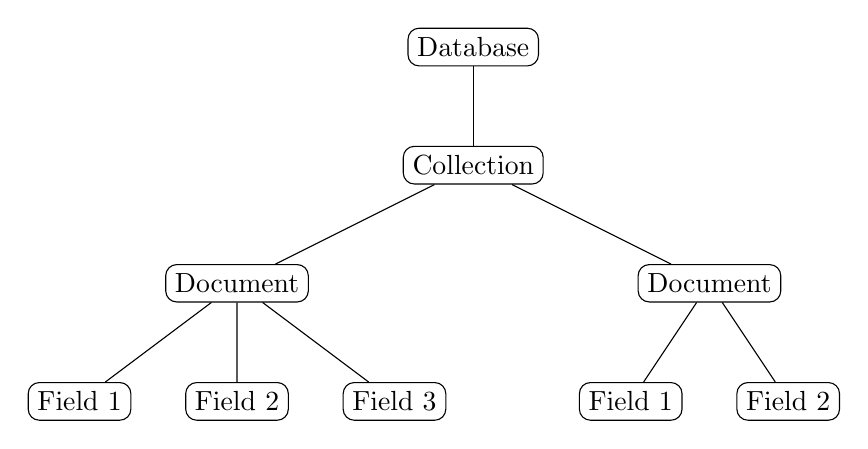
\begin{tikzpicture}[
		node distance=1.2cm,
		every node/.style={rectangle, draw=black, rounded corners, align=center, minimum height=1em},
		level 1/.style={sibling distance=6cm},
		level 2/.style={sibling distance=6cm},
		level 3/.style={sibling distance=2cm}
		]
		\node {Database}
		child { node {Collection}
			child { node {Document}
				child { node {Field 1} }
				child { node {Field 2} }
				child { node {Field 3} }
			}
			child { node {Document}
				child { node {Field 1} }
				child { node {Field 2} }
			}
		};
	\end{tikzpicture}
	\caption{Struktur Document Database: Database $\rightarrow$ Collection $\rightarrow$ Document $\rightarrow$ Fields}
	\label{fig:docdb_structure}
\end{figure}


Menurut \cite{moniruzzaman2013nosql}, keunggulan document database meliputi fleksibilitas tinggi dalam penyimpanan data, efisiensi penyimpanan data nested yang kompleks, serta kemudahan integrasi dengan aplikasi web modern melalui format JSON.

\subsection{Contoh dan Use Case}

\textbf{MongoDB} adalah document database paling populer di industri saat ini, didesain untuk mendukung penyimpanan data berskala besar dengan performa tinggi. MongoDB menyimpan dokumen dalam format BSON (Binary JSON), yang mendukung tipe data lebih beragam dibanding JSON standar \cite{mongodb2023doc}.

Contoh dokumen MongoDB untuk data produk e-commerce:

\begin{lstlisting}[language=json, caption={Contoh dokumen produk dalam MongoDB}, label={lst:mongodb_product}]
	{
		"_id": ObjectId("507f1f77bcf86cd799439011"),
		"name": "Laptop ASUS VivoBook",
		"category": "Electronics",
		"price": 8500000,
		"stock": 120,
		"specs": {
			"processor": "Intel i5",
			"ram": "8GB",
			"storage": "512GB SSD"
		},
		"tags": ["laptop", "asus", "notebook", "electronics"]
	}
\end{lstlisting}

\textbf{Contoh Query MongoDB}. MongoDB memiliki MongoDB Query Language (MQL) untuk melakukan pencarian dan manipulasi data. Contoh query berikut digunakan untuk menemukan semua produk dalam kategori "Electronics" dengan harga di bawah 10 juta rupiah:

\begin{lstlisting}[style=JavaScript, caption={Contoh query MongoDB untuk menemukan produk elektronik dengan harga < 10 juta}, label={lst:mongodb_query}]
	db.products.find(
	{ 
		category: "Electronics", 
		price: { $lt: 10000000 } 
	},
	{
		name: 1,
		price: 1,
		category: 1
	}
	);
\end{lstlisting}

Penjelasan query:
\begin{itemize}
	\item \texttt{db.products.find()}: mencari data pada collection \texttt{products}.
	\item \texttt{\{ category: "Electronics", price: \{ \$lt: 10000000 \} \}}: filter untuk kategori Electronics dan harga kurang dari 10 juta.
	\item \texttt{\{ name: 1, price: 1, category: 1 \}}: projection untuk hanya menampilkan nama, harga, dan kategori produk.
\end{itemize}

Dalam konteks bisnis, document database banyak digunakan untuk:
\begin{itemize}
	\item \textbf{Product catalogues}: struktur produk yang fleksibel dengan atribut bervariasi (mis. spesifikasi elektronik, buku, fashion).
	\item \textbf{User profiles}: data pengguna yang dinamis dengan preferensi, histori transaksi, dan metadata lainnya.
	\item \textbf{Content management systems (CMS)}: penyimpanan artikel, halaman web, atau konten digital lain dengan struktur tidak seragam.
	\item \textbf{Real-time analytics}: analisis data transaksi dengan skema yang terus berkembang.
\end{itemize}

Menurut \cite{gandomi2015}, penggunaan document database memungkinkan organisasi untuk mempercepat pengembangan aplikasi digital dan menyesuaikan struktur data dengan kebutuhan bisnis yang berubah cepat tanpa mengorbankan performa.

\subsection{Perbandingan RDBMS vs Document Database pada Kasus Produk Multikategori}

Pada aplikasi e-commerce yang menjual produk multikategori dengan atribut bervariasi seperti laptop, buku, fashion, dan furniture, terdapat perbedaan mendasar antara pendekatan RDBMS dan document database.

\paragraph{Pendekatan RDBMS (Schema-Based).}

Jika menggunakan RDBMS, tabel \texttt{products} didefinisikan dengan semua kolom atribut yang mungkin, seperti:

\begin{lstlisting}[style=SqlStyle]
	CREATE TABLE products (
	id INT PRIMARY KEY,
	name VARCHAR(100),
	category VARCHAR(50),
	price DECIMAL(10,2),
	screen_size VARCHAR(20),
	processor VARCHAR(30),
	ram VARCHAR(20),
	author VARCHAR(50),
	page_count INT,
	material VARCHAR(50),
	size VARCHAR(30)
	);
\end{lstlisting}

\textbf{Kendala yang muncul:}
\begin{itemize}
	\item Kolom seperti \texttt{screen\_size}, \texttt{processor}, \texttt{ram} hanya relevan untuk laptop, sedangkan \texttt{author}, \texttt{page\_count} hanya relevan untuk buku, dan \texttt{material}, \texttt{size} hanya relevan untuk furniture atau fashion, menyebabkan sebagian besar kolom berisi NULL.
	\item Menambahkan kategori produk baru dengan atribut unik (mis. sepatu dengan \texttt{shoe\_size}, kendaraan dengan \texttt{engine\_cc}) memerlukan \texttt{ALTER TABLE}, yang dapat memicu downtime dan migrasi skema yang kompleks pada sistem berskala besar.
	\item Query menjadi tidak optimal karena banyak kolom tidak relevan yang dibaca saat SELECT * dijalankan.
	\item Struktur rigid ini menghambat agility pengembangan ketika bisnis menambah kategori produk atau fitur baru dengan cepat.
\end{itemize}

\paragraph{Pendekatan Document Database (Schema-less, mis. MongoDB).}

Dengan document database, setiap produk disimpan sebagai dokumen dengan struktur atribut sesuai kategorinya.

\textbf{Contoh dokumen laptop:}

\begin{lstlisting}[language=json]
	{
		"name": "ASUS VivoBook",
		"category": "Electronics",
		"price": 8500000,
		"specs": {
			"screen_size": "15.6 inch",
			"processor": "Intel i5",
			"ram": "8GB"
		}
	}
\end{lstlisting}

\textbf{Contoh dokumen buku:}

\begin{lstlisting}[language=json]
	{
		"name": "Pemrograman Python Dasar",
		"category": "Book",
		"price": 95000,
		"author": "Budi Santoso",
		"page_count": 320
	}
\end{lstlisting}

\textbf{Contoh dokumen sepatu:}

\begin{lstlisting}[language=json]
	{
		"name": "Nike Air Max",
		"category": "Shoes",
		"price": 1200000,
		"shoe_size": "42 EU",
		"material": "Leather"
	}
\end{lstlisting}

\paragraph{Keunggulan Document Database pada Kasus Ini.}
\begin{itemize}
	\item \textbf{Tidak ada kolom kosong}. Setiap dokumen hanya menyimpan atribut yang relevan dengan produknya, mengoptimalkan penyimpanan dan efisiensi query.
	\item \textbf{Fleksibel dan agile}. Menambahkan kategori atau atribut baru tidak memerlukan perubahan skema collection atau downtime sistem.
	\item \textbf{Efisiensi query nested fields}. MongoDB mendukung indexing pada nested fields seperti \texttt{specs.screen\_size}, meningkatkan performa pencarian spesifikasi produk.
	\item \textbf{Developer friendly}. Format JSON/BSON sesuai dengan struktur data aplikasi web modern, mengurangi kebutuhan object-relational mapping.
	\item \textbf{Mendukung bisnis dinamis}. Perusahaan dapat menambahkan atau mengubah struktur produk dengan cepat sesuai kebutuhan pasar tanpa terhambat rigid schema.
\end{itemize}

\paragraph{Kelemahan Document Database pada Kasus Ini.}
\begin{itemize}
	\item \textbf{Kurang mendukung transaksi kompleks}. Jika aplikasi membutuhkan transaksi multi-dokumen dengan konsistensi ketat, RDBMS lebih optimal; misalnya ketika user melakukan checkout order, diperlukan update pada collection \texttt{orders} dan mengurangi stok pada collection \texttt{products}, dan tanpa dukungan transaksi multi-dokumen yang kuat terdapat risiko data tidak sinkron jika salah satu operasi gagal.
	
	\item \textbf{Tidak ada integrity constraints global}. Document DB tidak memiliki foreign key antar collection secara native, sehingga integritas data antar entitas harus dikelola di level aplikasi; contohnya memastikan \texttt{product\_id} yang direferensikan pada dokumen order benar-benar ada pada collection \texttt{products} harus divalidasi manual melalui kode aplikasi.
	
	\item \textbf{Query join terbatas}. Operasi agregasi data lintas collection tidak sefleksibel join SQL pada RDBMS; contohnya untuk menampilkan daftar order lengkap beserta detail user dan produk, pada RDBMS dapat menggunakan \texttt{JOIN}, sedangkan di document DB memerlukan multiple query atau data embedding yang meningkatkan duplikasi data.
	
	\item \textbf{Overhead storage}. Penyimpanan nested document yang besar dapat meningkatkan penggunaan disk dibanding data ter-normalisasi pada RDBMS; contohnya menyimpan spesifikasi laptop dan detail review user langsung dalam dokumen produk menyebabkan dokumen menjadi besar, padahal pada RDBMS data review dapat dipisah pada tabel tersendiri dan di-query hanya saat diperlukan.
\end{itemize}


\textbf{Kesimpulan}. Untuk kasus produk multikategori dengan struktur atribut yang heterogen dan sering berubah, \textbf{document database (schema-less)} seperti MongoDB lebih unggul dibanding RDBMS karena mendukung fleksibilitas skema dan pengembangan cepat. Namun, kelemahannya perlu dipertimbangkan, terutama jika aplikasi juga membutuhkan transaksi multi-entitas yang konsisten secara ACID dan integritas relasi antar tabel yang ketat.



\section{Graph Databases}

\subsection{Konsep dan Struktur}

\textbf{Graph database} adalah tipe NoSQL yang dirancang untuk menyimpan dan mengelola data yang terhubung atau memiliki relasi kompleks. Model data berbasis graf ini terdiri dari:
\begin{itemize}
	\item \textbf{Node}: merepresentasikan entitas (misalnya orang, produk, akun).
	\item \textbf{Edge}: merepresentasikan relasi antar node, misalnya “membeli”, “berteman dengan”, atau “merekomendasikan”.
	\item \textbf{Properties}: atribut yang dimiliki oleh node atau edge, misalnya nama, umur, harga, tanggal relasi.
\end{itemize}

Berbeda dengan basis data relasional yang menggunakan tabel dan join untuk menghubungkan data, graph database menyimpan relasi sebagai bagian inheren dari struktur data. Hal ini memungkinkan traversal atau penelusuran relasi yang sangat cepat tanpa memerlukan operasi join yang kompleks \cite{moniruzzaman2013nosql, han2011survey}. 

Menurut \cite{moniruzzaman2013nosql}, keunggulan utama graph database meliputi:
\begin{enumerate}
	\item Optimasi untuk query relasi kompleks dan traversal berlapis-lapis (multi-hop).
	\item Penyimpanan relasi secara langsung tanpa join, sehingga efisien untuk data terhubung.
	\item Fleksibilitas dalam menambahkan tipe node dan relasi baru tanpa perubahan skema global.
\end{enumerate}

\subsection{Contoh dan Use Case}


\textbf{Gambar \ref{fig:graphdb_structure}} berikut mengilustrasikan konsep dasar graph database, khususnya dalam skenario rekomendasi produk berdasarkan pembelian teman pengguna.

\begin{figure}[h]
	\centering
	\begin{tikzpicture}[->,>=stealth,shorten >=1pt,auto,
		thick,main node/.style={circle,draw,font=\sffamily\small\bfseries}]
		
		% Define nodes with custom positions for more spacing
		\node[main node] (1) {User};
		\node[main node] (2) [right=3.5cm of 1] {Friend};
		\node[main node] (3) [right=3.5cm of 2] {Product};
		
		\path[every node/.style={font=\sffamily\small}]
		(1) edge node [above] {FRIEND} (2)
		(2) edge node [above] {PURCHASED} (3);
	\end{tikzpicture}
	\caption{Struktur Graph Database: relasi User → Friend → Product untuk rekomendasi}
	\label{fig:graphdb_structure}
\end{figure}

\textbf{Neo4j} adalah graph database terpopuler di industri, menggunakan \textbf{property graph model} dengan Cypher Query Language (CQL) untuk menulis query berbasis pola relasi \cite{neo4j2023doc}.

Contoh query Cypher berikut digunakan untuk merekomendasikan produk berdasarkan pembelian yang dilakukan oleh teman pengguna bernama "Andi":

\begin{lstlisting}[style=SqlStyle, caption={Contoh query Cypher di Neo4j untuk rekomendasi produk berdasarkan pembelian teman}, label={lst:neo4j_recommend}]
	MATCH (user:User)-[:FRIEND]->(friend:User)-[:PURCHASED]->(product:Product)
	WHERE user.name = "Andi"
	RETURN DISTINCT product.name;
\end{lstlisting}

Penjelasan query:
\begin{itemize}
	\item \texttt{MATCH}: menelusuri pola relasi pada graph database.
	\item \texttt{(user:User)-[:FRIEND]->(friend:User)}: menemukan semua node \texttt{friend} yang memiliki relasi \texttt{FRIEND} dari \texttt{user}.
	\item \texttt{(friend)-[:PURCHASED]->(product:Product)}: menemukan produk yang dibeli oleh \texttt{friend}.
	\item \texttt{WHERE user.name = "Andi"}: memfilter agar hanya pengguna bernama Andi yang diproses.
	\item \texttt{RETURN DISTINCT product.name}: mengembalikan nama produk tanpa duplikasi.
\end{itemize}

Query seperti ini mendukung pembuatan \textbf{recommendation engine} dalam e-commerce, di mana produk yang dibeli teman pengguna dapat ditampilkan sebagai rekomendasi yang relevan dan personal.



Dalam konteks bisnis, graph database banyak digunakan untuk:
\begin{itemize}
	\item \textbf{Social networks}: menyimpan relasi pertemanan, pengikut (followers), dan interaksi antar pengguna.
	\item \textbf{Recommendation engines}: merekomendasikan produk berdasarkan pola pembelian pengguna lain dengan relasi serupa.
	\item \textbf{Fraud detection}: mendeteksi pola relasi mencurigakan dalam transaksi keuangan atau klaim asuransi.
	\item \textbf{Knowledge graph}: menghubungkan berbagai entitas dan konsep dalam domain tertentu untuk mendukung pencarian semantik.
\end{itemize}

Menurut \cite{gandomi2015}, kemampuan graph database dalam menganalisis relasi dan pola koneksi menjadikannya fondasi penting dalam pengembangan aplikasi berbasis jaringan dan analitik modern.


\subsection{Contoh Kasus Teknis: Keunggulan Graph Database}

Untuk memahami keunggulan graph database, berikut adalah contoh kasus nyata di mana penggunaan graph database lebih optimal dibanding RDBMS atau document database.

\subsubsection{Kasus: Rekomendasi Produk Berdasarkan Hubungan User}

\paragraph{Skenario.}

Sebuah platform e-commerce ingin menampilkan rekomendasi produk kepada user berdasarkan pembelian user lain yang memiliki preferensi atau hubungan sosial serupa (collaborative filtering). Struktur datanya meliputi:
\begin{itemize}
	\item User memiliki relasi pertemanan (friends).
	\item User melakukan pembelian produk (purchased).
	\item Produk memiliki kategori atau fitur tertentu.
\end{itemize}

\paragraph{Pendekatan RDBMS.}

Jika menggunakan RDBMS, data disimpan dalam tabel relasional seperti:

\begin{lstlisting}[style=SqlStyle]
	CREATE TABLE users (
	user_id INT PRIMARY KEY,
	name VARCHAR(100)
	);
	
	CREATE TABLE products (
	product_id INT PRIMARY KEY,
	name VARCHAR(100),
	category VARCHAR(50)
	);
	
	CREATE TABLE purchases (
	user_id INT,
	product_id INT,
	FOREIGN KEY (user_id) REFERENCES users(user_id),
	FOREIGN KEY (product_id) REFERENCES products(product_id)
	);
	
	CREATE TABLE friends (
	user_id INT,
	friend_id INT,
	FOREIGN KEY (user_id) REFERENCES users(user_id),
	FOREIGN KEY (friend_id) REFERENCES users(user_id)
	);
\end{lstlisting}

\textbf{Kendala RDBMS:}
\begin{itemize}
	\item Query untuk menemukan \textbf{“produk yang dibeli teman user”} membutuhkan multiple join (friends → purchases → products) yang kompleks dan lambat pada data besar.
	\item Setiap traversal relasi memerlukan join tambahan, meningkatkan kompleksitas query SQL dan waktu eksekusi.
\end{itemize}

\paragraph{Pendekatan Graph Database (mis. Neo4j).}

Dengan graph database, relasi antar data disimpan secara eksplisit sebagai edge antar node, mendukung traversal relasi yang cepat tanpa join tabel.

\textbf{Struktur node dan edge:}
\begin{itemize}
	\item Node: User, Product
	\item Edge: FRIEND, PURCHASED
\end{itemize}

\textbf{Contoh query Cypher untuk rekomendasi produk:}

\begin{lstlisting}[style=SqlStyle]
	MATCH (user:User)-[:FRIEND]->(friend:User)-[:PURCHASED]->(product:Product)
	WHERE user.name = "Andi"
	RETURN DISTINCT product.name;
\end{lstlisting}

\textbf{Keunggulan Graph Database dalam kasus ini:}
\begin{itemize}
	\item \textbf{Traversal multi-hop cepat}. Menemukan produk yang dibeli teman user hanya membutuhkan satu query pattern matching tanpa join tabel.
	\item \textbf{Model data intuitif}. Relasi user–friend–product dimodelkan langsung sebagai graph, mudah dipahami dan di-maintain.
	\item \textbf{Optimal untuk social recommendations}. Graph database dirancang khusus untuk analisis pola relasi (mis. shortest path, community detection, recommendations).
	\item \textbf{Scalability}. Neo4j mendukung jutaan node dan edge dengan performa traversal yang stabil.
\end{itemize}

\paragraph{Kelemahan Graph Database pada Kasus Ini.}
\begin{itemize}
	\item \textbf{Kurang optimal untuk operasi agregasi besar}. Graph database tidak dirancang untuk query agregasi seperti total sales per bulan; contohnya laporan penjualan bulanan tetap lebih cepat di RDBMS atau column store.
	
	\item \textbf{Overhead storage tinggi pada edge-heavy graph}. Menyimpan jutaan relasi (edge) membutuhkan storage dan memori besar dibanding tabel relasional terindex; contohnya social network dengan follower graph yang sangat dense.
	
	\item \textbf{Learning curve}. Penggunaan Cypher Query Language atau Gremlin memerlukan pembelajaran tambahan bagi tim yang terbiasa SQL; misalnya developer ERP tradisional perlu pelatihan untuk memahami pattern matching dan traversal.
	
	\item \textbf{Integrasi query lintas sistem}. Jika analitik memerlukan join data transaksi dari RDBMS dengan relasi graph di Neo4j, dibutuhkan pipeline ETL atau query federasi yang meningkatkan kompleksitas arsitektur.
\end{itemize}

\paragraph{Kesimpulan.}
Dalam kasus analisis relasi kompleks seperti social recommendations, fraud detection, atau supply chain network analysis, \textbf{graph database} lebih optimal dibanding RDBMS atau document database karena mendukung query traversal relasi berlapis-lapis dengan performa tinggi dan model data yang lebih natural.


\section{Key-Value Stores (Singkat)}

\subsection{Konsep dan Use Case}

\textbf{Key-Value Store} adalah tipe NoSQL paling sederhana yang menyimpan data sebagai pasangan \textbf{kunci (key)} dan \textbf{nilai (value)}. Konsepnya serupa dengan dictionary atau hash map dalam pemrograman, di mana:
\begin{itemize}
	\item \textbf{Key} berfungsi sebagai identifier unik.
	\item \textbf{Value} menyimpan data yang dapat berupa string, angka, JSON, atau binary blob.
\end{itemize}

Berbeda dengan database tradisional yang menyimpan data di disk secara default, banyak key-value store modern seperti \textbf{Redis} menggunakan \textbf{main memory (RAM)} sebagai media penyimpanan utama. Hal ini memungkinkan operasi baca dan tulis dilakukan dengan latensi yang sangat rendah (hampir real-time), menjadikannya ideal untuk aplikasi dengan kebutuhan performa tinggi \cite{moniruzzaman2013nosql}.

Namun, karena data disimpan di memori, muncul risiko kehilangan data ketika terjadi \textbf{power failure} atau restart server secara mendadak. Untuk mengatasi hal ini, Redis dan key-value store serupa menyediakan mekanisme \textbf{persistence} seperti:
\begin{enumerate}
	\item \textbf{Snapshotting}: secara berkala menyimpan salinan data dari memori ke disk dalam bentuk snapshot.
	\item \textbf{Append-Only File (AOF)}: mencatat setiap perubahan data ke file log di disk, sehingga data dapat di-replay saat recovery.
	\item \textbf{Hybrid}: kombinasi keduanya untuk trade-off antara durability dan performa.
\end{enumerate}

Meskipun demikian, persistensi ini dilakukan di background untuk menjaga performa operasi baca/tulis di memori. Konsekuensinya, masih terdapat risiko kehilangan data yang belum sempat tersimpan ke disk jika terjadi kegagalan sistem total secara tiba-tiba.

\textbf{Redis} adalah contoh key-value store paling populer. Selain menyimpan pasangan key-value sederhana, Redis juga mendukung struktur data kompleks seperti list, set, dan sorted set, yang memperluas use case dalam aplikasi modern.

Contoh use case key-value store dalam bisnis meliputi:
\begin{itemize}
	\item \textbf{Caching}: menyimpan hasil query atau halaman web yang sering diakses untuk mengurangi beban database utama dan meningkatkan kecepatan respon aplikasi.
	\item \textbf{Session store}: menyimpan session user dalam aplikasi web untuk mengelola autentikasi dan status login secara cepat.
	\item \textbf{Configuration management}: menyimpan konfigurasi aplikasi yang dibaca saat runtime.
	\item \textbf{Leaderboard atau ranking}: menggunakan sorted set Redis untuk aplikasi game atau e-commerce yang menampilkan peringkat produk atau pengguna.
\end{itemize}

Sebagai contoh penggunaan Redis untuk menyimpan session user:

\begin{lstlisting}[style=JavaScript, caption={Contoh perintah Redis untuk menyimpan session user}, label={lst:redis_session}]
	SET session: 12345 "{ \"user_id\": 789, \"login_time\": \"2025-06-27T10:00:00Z\" }"
\end{lstlisting}

Perintah di atas menyimpan data session dengan key \texttt{session:12345} dan value berupa JSON string berisi user ID dan waktu login.

Menurut \cite{gandomi2015}, penggunaan key-value store seperti Redis mendukung arsitektur aplikasi modern yang membutuhkan performa real-time, skalabilitas horizontal, dan responsivitas tinggi, meskipun organisasi perlu mempertimbangkan strategi persistence yang tepat untuk memastikan durability data sesuai kebutuhan bisnis.



\section{Perbandingan NoSQL dan RDBMS}

\textbf{Relational Database Management System (RDBMS)} dan \textbf{NoSQL} memiliki peran strategis yang berbeda dalam pengelolaan data modern. Pemahaman perbedaan keduanya penting dalam merancang sistem bisnis yang efektif, efisien, dan scalable.

\subsection{Karakteristik Utama}

Perbedaan mendasar antara RDBMS dan NoSQL terletak pada cara penyimpanan data, skema, dan arsitektur skalabilitasnya. RDBMS menggunakan pendekatan tabel relasional dengan skema tetap yang memastikan konsistensi dan integritas data, sedangkan NoSQL mendukung format data yang lebih fleksibel untuk kebutuhan big data modern dan aplikasi real-time. \textbf{Tabel~\ref{tab:rdbms_nosql_comparison}} berikut merangkum karakteristik utama keduanya sebagai dasar pemahaman sebelum menentukan pilihan implementasi dalam sistem bisnis.

\begin{table}[h]
	\centering
	\renewcommand{\arraystretch}{1.3}
	\caption{Perbandingan RDBMS dan NoSQL}
	\label{tab:rdbms_nosql_comparison}
	\begin{tabular}{|p{0.18\textwidth}|p{0.27\textwidth}|p{0.47\textwidth}|}
		\hline
		\textbf{Aspek} & \textbf{RDBMS} & \textbf{NoSQL} \\
		\hline
		Struktur data & Tabel relasional dengan skema tetap & Beragam (document, key-value, columnar, graph) dengan skema fleksibel \\
		\hline
		Skema & Rigid (schema-first) & Fleksibel (schema-less atau schema-later) \\
		\hline
		Query Language & SQL standar (SELECT, JOIN) & Query language bervariasi sesuai tipe NoSQL (mis. MQL di MongoDB, CQL di Cassandra) \\
		\hline
		Transaksi & Mendukung ACID (Atomicity, Consistency, Isolation, Durability) penuh & Dominan BASE (Basically Available, Soft state, Eventually consistent), namun beberapa mendukung transaksi terbatas \\
		\hline
		Skalabilitas & Vertikal (meningkatkan kapasitas server) & Horizontal (menambah node pada cluster) \\
		\hline
		Use case utama & Sistem transaksi bisnis (OLTP), ERP, CRM & Big data, real-time analytics, IoT, social networks, content management \\
		\hline
	\end{tabular}
\end{table}


\subsection{Kelebihan dan Kelemahan}

\textbf{RDBMS}
\begin{itemize}
	\item \textbf{Kelebihan}: Konsistensi data terjamin, standar industri yang matang, mendukung transaksi kompleks dengan integrity constraints (mis. foreign key).
	\item \textbf{Kelemahan}: Kurang fleksibel untuk data semi-struktur, kurang optimal untuk skala horizontal (distributed systems).
\end{itemize}

\textbf{NoSQL}
\begin{itemize}
	\item \textbf{Kelebihan}: Skalabilitas horizontal tinggi, mendukung skema fleksibel untuk data semi-struktur atau tidak terstruktur, cocok untuk big data dan real-time application.
	\item \textbf{Kelemahan}: Tidak semua mendukung ACID transactions, query language bervariasi sehingga memerlukan learning curve, dan consistency trade-off (eventual consistency) perlu diperhatikan pada sistem yang memerlukan data akurat real-time.
\end{itemize}

\subsection{Implikasi Strategis bagi Sistem Bisnis}

Pemilihan antara RDBMS dan NoSQL memiliki dampak strategis pada desain sistem bisnis:

\begin{enumerate}
	\item \textbf{Stabilitas dan Integritas Transaksi}: Untuk aplikasi yang memerlukan integritas transaksi tinggi (mis. perbankan, akuntansi, ERP), RDBMS tetap menjadi pilihan utama karena mendukung ACID secara penuh.
	\item \textbf{Skalabilitas dan Kecepatan Respons}: NoSQL unggul dalam skenario dengan data volume sangat besar, kebutuhan low latency, atau akses paralel oleh jutaan pengguna seperti social media dan e-commerce besar.
	\item \textbf{Fleksibilitas Skema}: NoSQL mendukung agile development dengan perubahan skema data yang cepat tanpa perlu migrasi tabel kompleks, cocok untuk startup dan proyek dengan evolving data model.
	\item \textbf{Hybrid Architecture}: Banyak organisasi mengimplementasikan keduanya. RDBMS digunakan untuk core transaction systems sedangkan NoSQL untuk caching, big data analytics, dan real-time application layer \cite{gandomi2015, moniruzzaman2013nosql}.
\end{enumerate}

Menurut \cite{gandomi2015}, tren big data mendorong adopsi NoSQL untuk menangani variety dan velocity data yang tidak dapat diakomodasi RDBMS secara optimal. Namun, RDBMS tetap dominan sebagai tulang punggung sistem transaksi yang membutuhkan consistency dan reliability tinggi.


\section{Fleksibilitas Desain Skema}

Desain skema merupakan salah satu aspek terpenting dalam pengelolaan basis data karena menentukan bagaimana data disimpan, diakses, dan dimodifikasi. Pada RDBMS tradisional, desain skema bersifat \textbf{schema-based} atau rigid, sedangkan pada banyak NoSQL database, desainnya bersifat \textbf{schema-less} atau fleksibel.

\subsection{Schema-Based (Rigid Schema)}

Dalam RDBMS, sebelum data dapat dimasukkan, skema tabel harus didefinisikan secara eksplisit dengan tipe data dan constraints yang ketat. Pendekatan ini memiliki kelebihan:
\begin{itemize}
	\item Menjamin konsistensi data karena setiap record mematuhi struktur dan tipe yang sudah ditentukan.
	\item Memudahkan integrasi antar tabel melalui foreign key dan relasi relasional yang kuat.
	\item Mendukung validasi data dan transaksi yang memerlukan integritas tinggi.
\end{itemize}

Namun, rigid schema juga memiliki keterbatasan:
\begin{itemize}
	\item Perubahan struktur tabel (mis. penambahan kolom) membutuhkan migrasi skema yang kompleks.
	\item Kurang fleksibel untuk data dengan variasi atribut yang tinggi atau data semi-terstruktur seperti log dan JSON.
\end{itemize}

\subsection{Schema-less (Flexible Schema)}

Sebaliknya, banyak NoSQL database seperti MongoDB dan Cassandra mendukung desain \textbf{schema-less}, di mana data dapat disimpan tanpa mendefinisikan struktur kolom sebelumnya. Kelebihan pendekatan schema-less meliputi:
\begin{itemize}
	\item \textbf{Fleksibilitas tinggi}: setiap dokumen atau record dapat memiliki atribut berbeda sesuai kebutuhan.
	\item \textbf{Agile adaptation}: mendukung pengembangan aplikasi yang cepat dan iteratif tanpa downtime akibat migrasi skema.
	\item \textbf{Cocok untuk data semi-terstruktur}: seperti JSON, XML, log data, dan metadata variatif.
\end{itemize}

Contohnya pada MongoDB, dokumen untuk produk elektronik dan buku dapat memiliki field yang berbeda dalam collection yang sama, sesuai kebutuhan bisnis.


\subsection{Manfaat Fleksibilitas untuk Adaptasi Bisnis}

Dalam konteks bisnis modern yang dinamis, kemampuan untuk beradaptasi dengan cepat terhadap perubahan pasar, regulasi, dan kebutuhan pelanggan adalah faktor strategis. Desain schema-less mendukung:
\begin{enumerate}
	\item Percepatan pengembangan fitur baru tanpa kendala rigid schema.
	\item Integrasi data dari berbagai sumber heterogen tanpa ETL kompleks.
	\item Eksperimen bisnis dan data product development dengan time-to-market lebih singkat.
\end{enumerate}

Menurut \cite{gandomi2015}, fleksibilitas skema menjadi salah satu kunci competitive advantage pada era big data dan digital transformation.

\subsection{Risiko Poor Data Governance}

Namun, fleksibilitas schema-less juga membawa risiko signifikan jika tidak diimbangi dengan data governance yang baik:
\begin{itemize}
	\item \textbf{Inconsistent data structure}: variasi field antar dokumen dapat menyulitkan query, analitik, dan integrasi downstream.
	\item \textbf{Data quality issues}: tanpa constraint, data yang tidak valid atau tidak standar lebih mudah tersimpan.
	\item \textbf{Technical debt}: semakin banyak variasi struktur data tanpa pengelolaan dapat menyebabkan kerumitan dalam maintenance di masa depan.
\end{itemize}

Oleh karena itu, meskipun schema-less mendukung agility, organisasi tetap perlu menetapkan \textbf{data standards, validation rules, dan governance policies} yang jelas untuk memastikan kualitas dan integritas data tetap terjaga di seluruh sistem bisnis.



\section{Jenis-Jenis Database dan Relevansi Bisnis}

Pemilihan tipe database yang tepat sangat penting untuk memastikan sistem informasi mendukung kebutuhan bisnis secara optimal. Berikut adalah jenis-jenis database yang umum digunakan di industri beserta tujuan, skenario optimal, dan relevansinya dalam konteks bisnis modern.

\begin{longtable}{|p{0.11\textwidth}|p{0.21\textwidth}|p{0.21\textwidth}|p{0.35\textwidth}|}
	\hline
	\textbf{Jenis Database} & \textbf{Tujuan Utama} & \textbf{Skenario Optimal} & \textbf{Relevansi Bisnis} \\
	\hline
	\endfirsthead
	\hline
	\textbf{Jenis Database} & \textbf{Tujuan Utama} & \textbf{Skenario Optimal} & \textbf{Relevansi Bisnis} \\
	\hline
	\endhead
	
	Relational DB (RDBMS) & Penyimpanan data terstruktur dengan transaksi yang konsisten & OLTP systems, ERP, CRM & Mengelola transaksi bisnis, akuntansi, dan integritas data antar unit bisnis \\
	\hline
	
	Document DB & Penyimpanan data semi-struktur dengan skema fleksibel & Product catalogues, user profiles, content management & Mendukung variasi produk atau konten yang cepat berubah tanpa perlu migrasi skema \\
	\hline
	
	Key-Value Store & Penyimpanan data sederhana dengan kecepatan sangat tinggi & Caching, session store, real-time config & Meningkatkan performa aplikasi dengan mengurangi load ke database utama \\
	\hline
	
	Column-based DB & Penyimpanan kolom terpisah untuk query agregasi cepat & Data warehouse, analytics, time-series data & Mendukung analitik kompleks dan laporan manajemen dengan kecepatan tinggi \\
	\hline
	
	Graph DB & Penyimpanan relasi antar entitas dengan efisien & Social networks, recommendation engines, fraud detection & Memahami hubungan antar entitas untuk rekomendasi produk atau deteksi penipuan \\
	\hline
	
	Time-Series DB & Penyimpanan data berurutan dengan timestamp & Sensor IoT, financial tick data, monitoring metrics & Analisis tren data waktu nyata (real-time monitoring, prediksi harga saham) \\
	\hline
	
	Search Engine DB & Penyimpanan dan indexing teks untuk pencarian cepat & Full-text search, product search, document search & Meningkatkan user experience melalui pencarian cepat dan relevan di e-commerce atau portal berita \\
	\hline
	
	In-Memory DB & Penyimpanan data di RAM untuk kecepatan ultra tinggi & Real-time analytics, session caching, gaming leaderboards & Mendukung aplikasi yang membutuhkan response time sub-millisecond (ultra-low latency) \\
	\hline
	
	Ledger DB & Penyimpanan transaksi immutable dengan integritas tinggi & Financial records, blockchain, audit trails & Menjamin keamanan dan keaslian data transaksi untuk kebutuhan regulasi dan audit \\
	\hline
	
	Multi-Model DB & Mendukung beberapa model data dalam satu sistem & Hybrid applications, data integration platforms & Fleksibilitas tinggi untuk aplikasi yang membutuhkan kombinasi relasional, document, dan graph dalam satu platform \\
	\hline
	
\end{longtable}

\textbf{Penjelasan tambahan:}

\begin{itemize}
	\item \textbf{Relational DB (RDBMS)} seperti Oracle, MySQL, dan PostgreSQL tetap menjadi tulang punggung sistem transaksi bisnis dengan kebutuhan konsistensi tinggi.
	\item \textbf{Document DB} seperti MongoDB unggul untuk aplikasi dengan variasi data yang tinggi, misalnya katalog e-commerce.
	\item \textbf{Key-Value Store} seperti Redis mendukung caching dan session management untuk performa tinggi.
	\item \textbf{Column-based DB} seperti Apache Cassandra dan Google Bigtable dioptimalkan untuk analitik dengan data besar.
	\item \textbf{Graph DB} seperti Neo4j ideal untuk model hubungan kompleks, misalnya social media atau supply chain network.
	\item \textbf{Time-Series DB} seperti InfluxDB fokus pada data sensor dan metrik waktu.
	\item \textbf{Search Engine DB} seperti Elasticsearch mengoptimalkan full-text search dengan relevansi tinggi.
	\item \textbf{In-Memory DB} seperti Redis dan SAP HANA digunakan untuk kebutuhan komputasi ultra cepat.
	\item \textbf{Ledger DB} seperti Amazon QLDB atau Hyperledger Fabric digunakan untuk pencatatan transaksi immutable.
	\item \textbf{Multi-Model DB} seperti ArangoDB mendukung fleksibilitas tinggi dengan beberapa paradigma data dalam satu engine.
\end{itemize}

Pemahaman jenis-jenis database ini mendukung pengambilan keputusan strategis dalam perancangan arsitektur data perusahaan sesuai kebutuhan performa, skala, dan kompleksitas bisnis modern.



\section{Studi Kasus Singkat}

Pemahaman konsep dan jenis database akan lebih konkret ketika diterapkan dalam konteks kasus nyata. Berikut adalah studi kasus singkat untuk membantu mahasiswa memahami pertimbangan memilih antara RDBMS, Document DB, dan Graph DB.

\subsection{Skenario Bisnis}

\textbf{Perusahaan E-Commerce Multikategori}

Sebuah perusahaan e-commerce menjual berbagai produk seperti elektronik, fashion, buku, dan perlengkapan rumah tangga. Sistem mereka membutuhkan:

\begin{enumerate}
	\item \textbf{Transaksi Penjualan (Order Management)}  
	Pencatatan transaksi pembelian user, pembayaran, dan pengelolaan stok produk dengan integritas data tinggi.
	
	\item \textbf{Katalog Produk yang Bervariasi}  
	Setiap kategori produk memiliki atribut berbeda. Contoh, produk elektronik memiliki spesifikasi teknis (CPU, RAM), buku memiliki penulis dan jumlah halaman, fashion memiliki ukuran dan warna.
	
	\item \textbf{Rekomendasi Produk Berdasarkan Hubungan Pembelian dan Preferensi}  
	Perusahaan ingin menampilkan rekomendasi produk berdasarkan pembelian user lain yang memiliki preferensi serupa (mis. collaborative filtering).
\end{enumerate}

\subsection{Pilihan Database dan Analisis}

Untuk menentukan database yang optimal pada sistem e-commerce multikategori, \textbf{Tabel~\ref{tab:db_choice_analysis}} berikut merangkum analisis pilihan berdasarkan kebutuhan utama.

\begin{table}[h]
	\centering
	\renewcommand{\arraystretch}{1.3}
	\caption{Pilihan Database untuk Modul Sistem E-Commerce Multikategori}
	\label{tab:db_choice_analysis}
	\begin{tabular}{|
			p{0.15\textwidth}|
			p{0.20\textwidth}|
			>{\raggedright\arraybackslash}p{0.55\textwidth}|
		}
		\hline
		\textbf{Modul/Kebutuhan} & \textbf{Database Pilihan} & \textbf{Alasan Teknis dan Bisnis} \\
		\hline
		Transaksi Penjualan & RDBMS (PostgreSQL, MySQL) &
		- Mendukung transaksi ACID untuk pembayaran, stok, dan order dengan integritas tinggi. \newline
		- Struktur data homogen dan relasi antar tabel jelas (order, payment, inventory). \\
		\hline
		Katalog Produk Multikategori & Document DB (MongoDB) &
		- Setiap produk memiliki atribut berbeda tanpa alter table. \newline
		- Mendukung nested data (mis. spesifikasi elektronik). \newline
		- Fleksibel untuk penambahan kategori atau atribut produk baru tanpa downtime. \\
		\hline
		Rekomendasi Produk & Graph DB (Neo4j) &
		- Menyimpan dan memproses relasi user dan produk dengan efisien. \newline
		- Mendukung query berbasis pola relasi (mis. collaborative filtering). \newline
		- Optimal untuk analisis social graph dan rekomendasi personalisasi. \\
		\hline
	\end{tabular}
\end{table}


\subsection{Rekomendasi Strategis}

Berdasarkan analisis pada \textbf{Tabel~\ref{tab:db_choice_analysis}}, pendekatan arsitektur data yang disarankan adalah \textbf{polyglot persistence}, yaitu menggunakan beberapa tipe database secara bersamaan untuk mengoptimalkan fungsi masing-masing:

\begin{enumerate}
	\item \textbf{RDBMS} untuk transaksi penjualan dan integritas data finansial (ERP core).
	\item \textbf{Document DB} untuk katalog produk dengan struktur dinamis dan heterogen.
	\item \textbf{Graph DB} untuk engine rekomendasi berbasis relasi user dan produk.
\end{enumerate}

Pendekatan ini mendukung performa tinggi dan agility sistem. Menurut \cite{gandomi2015}, strategi polyglot persistence merupakan praktik umum pada arsitektur big data modern untuk memenuhi kebutuhan scalability, flexibility, dan reliability secara simultan.

\section{Other Aspects to Consider in Database Selection}

Selecting a database system is not only a technical decision but also involves strategic business considerations. Beyond data structure, schema flexibility, and scalability, organisations need to evaluate the following aspects to ensure effective and sustainable implementation:

\subsection{Cost and Licensing}

Cost considerations include:
\begin{itemize}
	\item \textbf{Licensing Model:} Commercial RDBMS (e.g. Oracle, SQL Server) may incur significant licence fees per CPU or user, while open-source alternatives (e.g. PostgreSQL, MongoDB Community) reduce upfront costs.
	\item \textbf{Operational Cost:} Includes infrastructure, maintenance, and backup strategies, especially for distributed NoSQL clusters requiring multiple nodes.
	\item \textbf{Total Cost of Ownership (TCO):} Evaluates long-term expenses including scaling, support contracts, training, and cloud subscription fees.
\end{itemize}

\subsection{Vendor Lock-In Risk}

Dependence on proprietary database features may:
\begin{itemize}
	\item Limit flexibility to migrate to other vendors in the future.
	\item Increase switching costs due to incompatibility with standard SQL or lack of equivalent features in other platforms.
	\item Influence negotiation power with the vendor, especially for critical business applications.
\end{itemize}

\subsection{Human Resource Skills and Training}

Successful database adoption depends on the available skills within the organisation:
\begin{itemize}
	\item RDBMS expertise is widely available but optimising NoSQL requires specialised knowledge of data models, consistency trade-offs, and distributed system design.
	\item Training costs and learning curves for new query languages (e.g. Cypher, Gremlin) must be considered in project timelines and budgets.
\end{itemize}

\subsection{Integration with Existing Systems}

Compatibility with existing applications, middleware, and data pipelines influences database choice:
\begin{itemize}
	\item RDBMS integrates well with legacy ERP and financial systems.
	\item NoSQL may require additional connectors or ETL tools for integration with BI platforms or reporting tools.
\end{itemize}

\subsection{Compliance and Security}

Industry standards and data governance requirements may dictate:
\begin{itemize}
	\item Support for encryption at rest and in transit.
	\item Compliance with data protection regulations (e.g. GDPR, HIPAA).
	\item Audit logging capabilities for security monitoring and regulatory audits.
\end{itemize}

\subsection{Community Support and Ecosystem}

Strong community and ecosystem support ensure:
\begin{itemize}
	\item Faster problem resolution and access to best practices.
	\item Availability of third-party tools, drivers, and libraries for development.
\end{itemize}

\vspace{10pt}
Considering these non-technical aspects alongside technical fit will help organisations make holistic decisions aligning with business objectives, resource capacity, and long-term data strategy.


\section{Kesimpulan}

Dalam era big data dan transformasi digital saat ini, kebutuhan akan penyimpanan data yang fleksibel, scalable, dan mendukung berbagai format data mendorong organisasi untuk mempertimbangkan penggunaan \textbf{NoSQL} di samping RDBMS tradisional. NoSQL hadir untuk menjawab tantangan yang tidak dapat diselesaikan RDBMS secara optimal, seperti penanganan data semi-struktur dan tidak terstruktur (misalnya JSON, XML), kebutuhan latensi rendah pada real-time application, serta skalabilitas horizontal untuk mendukung jutaan transaksi atau interaksi pengguna secara bersamaan. Dengan berbagai kategorinya seperti document database, key-value store, column-family store, dan graph database, NoSQL menawarkan pilihan teknologi yang dapat disesuaikan dengan karakteristik data dan pola akses pada setiap use case bisnis.\\

Namun, keputusan untuk mengimplementasikan NoSQL harus didasarkan pada pertimbangan strategis yang matang. RDBMS tetap unggul dalam transaksi bisnis yang membutuhkan integritas data dan konsistensi tinggi (ACID). Sebaliknya, NoSQL memberikan keunggulan pada aspek agility, time-to-market, serta kemampuan mengelola data dengan struktur dinamis dalam ekosistem digital modern. Oleh karena itu, banyak organisasi mengadopsi pendekatan \textbf{polyglot persistence}, yaitu kombinasi RDBMS dan NoSQL, untuk mengoptimalkan kekuatan masing-masing teknologi sesuai kebutuhan modul dan fungsi bisnis. Pemahaman mendalam terhadap kelebihan, keterbatasan, serta relevansi bisnis dari setiap jenis database akan membantu para manajer, arsitek sistem, dan pengambil keputusan dalam merancang arsitektur data yang efektif dan kompetitif di era digital.